\section{Integration}
\subsection{The Riemann Integral}
Our goal is the following: for a ``sufficiently nice'' function $f:[a,b]\to\mathbb R$ we want to define its integral
$$\int_a^bf(x)\,\mathrm dx$$
We would like to think of this as the area under the graph of $y=f(x)$, which motivates the Riemann integral.
\begin{definition}
    $f:[a,b]\to \mathbb{R}$ is called \textbf{bounded} if $ \exists K,\ \forall x\in [a,b],\ |f(x)|\le K $. 
\end{definition}
\begin{definition}
    A dissection(or partition) of the interval $[a,b]$ is a finite subset $D\subseteq [a,b]$ such that $a,b\in D$.
    If $D$ is a dissection, we can write $D=\{a_0,\ldots,a_n\}$ where $a=a_0<a_1<\cdots<a_n=b$.
\end{definition}
Note that if $D,D'$ are both dissections, so is $D\cup D'$.
\begin{definition}
    If $f:[a,b]\to\mathbb R$ is bounded and a dissection $D$ consists of $a=a_0<a_1<\cdots<a_n=b$, then we define the \textbf{upper} and \textbf{lower} \textbf{Riemann sums} wrt $D$ by
    respectively.
    \begin{align*}
        U(f,D)&=\sum_{i=1}^n(a_i-a_{i-1})\sup_{x\in [a_{i-1},a_i]}f(x),\\ 
        L(f,D)&=\sum_{i=1}^n(a_i-a_{i-1})\inf_{x\in [a_{i-1},a_i]}f(x).
    \end{align*}
    They exists as $f$ is bounded.
\end{definition}
Clearly $ L(f,D)\le U(f,D),\ \forall D $.
\begin{lemma}\label{lma:5.1}
    If $D\subseteq D'$ are dissections of $[a,b]$, then 
    \[
        U(f,D)\ge U(f,D')\ge L(f,D')\ge L(f,D).
    \]
\end{lemma}
\begin{proof}
    $U(f,D')\ge L(f,D')$ is obvious. Suppose $ D' $ contains an extra point than $D$, say $ y\in (x_{r-1},x_r) $. Clearly 
    \[
        \sup_{x\in [x_{r-1},y]}f(x),\sup_{x\in [y,x_r]}f(x)\le \sup_{x\in [x_{r-1},x_r]}f(x),
    \]
    so 
    \[
        (x_r-x_{r-1})\sup_{x\in [x_{r-1},x_r]}f(x)\ge (y-x_{r-1})\sup_{x\in [x_{r-1},y]}f(x)+(x_r-y)\sup_{x\in [y,x_r]}f(x).
    \]
    Summing over gives the result. Similarly for $D'$ with more extra points and $ L $.
\end{proof}
\begin{lemma}
    If $D_1,D_2$ are dissections of $[a,b]$, then
    \[
        U(f,D_1)\ge U(f,D_1 \cup D_2)\ge L(f,D_1 \cup D_2)\ge L(f,D_2).
    \]
\end{lemma}
\begin{proof}
    Take $ D'=D_1 \cup D_2 $ in the previous lemma.
\end{proof}

\begin{definition}
    The \textbf{upper integral} of $f$ is defined as 
    \[
        U(f) = \inf_D U(f,D),
    \]
    and the \textbf{lower integral} of $f$ is defined as 
    \[
        L(f) = \sup_D L(f,D).
    \]
    They both exists since $ U(f,D),L(f,D) $ are bounded.
\end{definition}
Hence 
\begin{sprop}
    $U(f)\ge L(f)$.
\end{sprop}

\begin{definition}
    A bounded function $ f:[a,b]\to \mathbb{R}  $ is said to be \textbf{Riemann integrable} on $[a,b]$ if $ U(f)=L(f) $ and we set
    $$\int_a^bf(x)\,\mathrm dx=L(f)=U(f) = \int_{a}^{b} f.$$
\end{definition}
\begin{example}\
    \begin{enumerate}
        \item Consider $f(x)=c$ for a constant $c$ for all $x\in [a,b]$, then consider $D=\{a,b\}$, then $U(f,D)=c(b-a)=L(f,D)$, hence $U(f)=c(b-a)=L(f)$, therefore $f$ is Riemann integrable and
        $$\int_a^bf(x)\,\mathrm dx=c(b-a).$$
        \item $f:[a,b]\to\mathbb R$ by $f(x)=0$ if $x\in\mathbb Q$ and $f(x)=1$ if $x\in\mathbb R\setminus\mathbb Q$. Note that if $a_{i-1}<a_i$, then $[a_{i-1},a_i]$ contains both rational and irrational numbers, so it follows that $U(f,D)=b-a$ and $L(f,D)=0$ for any dissection $D$ of $[a,b]$, therefore $U(f)=b-a\neq 0=L(f)$, hence $f$ is not Riemann integrable.
    \end{enumerate}
\end{example}

\subsection{Properties of riemann integrals}
\begin{theorem}\label{thm:5.3}
    Bounded $f:[a,b]\to\mathbb R$ is Riemann integrable on $[a,b]$ if and only if for every $\epsilon>0$, there is a dissection $D$ of $[a,b]$ such that 
    \[
        U(f,D)-L(f,D)<\epsilon.
    \]
\end{theorem}
\begin{proof}
    For every dissection $ D $ we have 
    \[
        0\le U(f)-L(f)\le U(f,D)-L(f,D).
    \]
    If the given condition holds, then 
    \[
        0\le U(f)-L(f)\le U(f,D)-L(f,D)<\epsilon,\quad \forall \epsilon>0.
    \]
    Immediately, $ L(f)=U(f) $.

    Suppose conversely $ f $ is integrable, by definition of $ \sup ,\inf  $, $ \exists D_1,D_2 $ such that 
    \begin{align*}
        &\int_{a}^{b} f(x) \,\mathrm{d}x -\frac{\epsilon}{2} = L(f)-\frac{\epsilon}{2} < L(f,D_1),\\ 
        &U(f,D_2)<U(f)+\frac{\epsilon}{2}=\int_{a}^{b} f(x) \,\mathrm{d}x+\frac{\epsilon}{2}.
    \end{align*}
    By lemma \ref{lma:5.1}, 
    \[
        U(f,D_1 \cup D_2)-L(f,D_1 \cup D_2)\le U(f,D_2)-L(f,D_1)<\epsilon.
    \]
\end{proof}
\begin{theorem}\label{thm:5.4}
    If $ f:[a,b]\to \mathbb{R} $ is monotonic, then $f$ is integrable.
\end{theorem}
\begin{proof}
    Wlog suppose $ f \nearrow $. Then
    \[
        \sup_{x\in [x_{j-1},x_j]}f(x)=f(x_j)\quad \text{and}\quad \inf_{x\in [x_{j-1},x_j]}f(x)=f(x_{j-1}).
    \]
    Thus 
    \[
        U(f,D)-L(f,D) = \sum_{j=1}^{n}(x_j-x_{j-1})[f(x_j)-f(x_{j-1})].
    \]
    Now consider 
    \[
        D = \left\{ a,a+\frac{b-a}{n},\dots,b \right\}.
    \]
    We have 
    \[
        U(f,D)-L(f,D)=\frac{b-a}{n}(f(b)-f(a)).
    \]
    Take $n$ large enough so that $ U(f,D)-L(f,D)<\epsilon $, and use theorem \ref{thm:5.3}
\end{proof}
\begin{definition}[Uniform continuity]
    $ f:[a,b]\to \mathbb{R} $ is called \textbf{uniformly continuous} if $ \forall \epsilon>0,\ \exists \delta>0,\ \forall x,y\in [a,b],\ |x-y|<\delta \Rightarrow |f(x)-f(y)|<\epsilon $.
\end{definition}
\begin{lemma}\label{lma:5.5}
    If $ f:[a,b]\to \mathbb{R}  $ is continuous, then it is uniformly continuous.
\end{lemma}
\begin{proof}[Proof by contradiction.]
    Suppose the claim is false. Then $ \exists \epsilon>0,\ \forall \delta>0,\ \exists x,y\in [a,b],\ |x-y|<\delta $ but $ |f(x)-f(y)|\ge \epsilon $. Take $ \delta=1/n $ to get $ x_n,y_n $ with such property. By Bolzano-Weierstrass, $ \exists x_{n_k}\to c $. Note that 
    \[
        |y_{n_k}-c|\le |y_{n_k}-x_{n_k}|+|x_{n_k}-c|\to 0 \Longleftrightarrow y_{n_k}\to c,
    \]
    but $ |f(x_{n_k})-f(y_{n_k})|\ge \epsilon $. Let $ k\to \infty $, by continuity, $ |f(x_{n_k})-f(y_{n_k})|\to 0 $, \#.
\end{proof}

\begin{theorem}\label{thm:5.6}
    Let $f:[a,b]\to \mathbb{R}$ be continuous, then $f$ is integrable. 
\end{theorem}
\begin{proof}
    By lemma, $ \forall \epsilon>0,\ \exists \delta>0,\ \forall x,y\in [a,b],\ |x-y|<\delta \Rightarrow |f(x)-f(y)|<\epsilon $. Let 
    \[
        D=\left\{ a+\frac{(b-a)j}{n}:j=0,\dots,n \right\}.
    \]
    Choose $n$ large so that $ (b-a)/n<\delta $. Then $\forall  x,y\in [x_{j-1},x_j] $, $ |f(x)-f(y)|<\epsilon $. This means that 
    \[
        \max_{x\in [x_{j-1},x_j]}f(x)-\min _{x\in [x_{j-1},x_j]}f(x)=f(p)-f(q),\quad p,q\in[x_{j-1},x_j]
    \]
    by continuity. Now 
    \begin{align*}
        U(f,D)-L(f,D)&= \sum_{j=1}^{n}(x_{j}-x_{j-1})\left( \max_{x\in [x_{j-1},x_j]}f(x)-\min _{x\in [x_{j-1},x_j]}f(x) \right)\\ 
        &= \sum_{j=1}^{n}\frac{(b-a)}{n}(f(p_j)-f(q_j))\\ 
        &<\epsilon(b-a).
    \end{align*}
    Hence $f$ is integrable by theorem \ref{thm:5.3}.
\end{proof}
\begin{example}
    Let $ f:[0,1]\to \bbR $ be defined by 
    \[
        f(x) = \begin{cases}
        1/q & x = p/q \text{ in lowest form}\\
        0 &\text{otherwise}\\
        \end{cases} 
    \]
    Clearly $ L(f,D)=0,\ \forall D $. We will show that $ \forall \epsilon>0,\ \exists D,\ U(f,D)<\epsilon $. This implies $f$ is integrable with 
    \[
        \int_{0}^{1} f(x) \,\mathrm{d}x=0.
    \]
    Take $ N\in \mathbb{N} $ such that $ 1/N<\epsilon/2 $. Consider 
    \[
        \{x\in [0,1]: f(x)\ge 1/N\} = \{p/q:1\le q\le N \land 1\le p\le q\}.
    \]
    This is a finite set with $ 0<t_1<\cdots<t_R=1 $. Consider $D$ such that 
    \begin{enumerate}
        \item Each $ t_k $ is in some interval $ [x_{j-1},x_j] $.
        \item $ \forall k $, the unique interval contaning $t_k$ has length at most $ \epsilon/2. $
    \end{enumerate}
    \begin{center}
        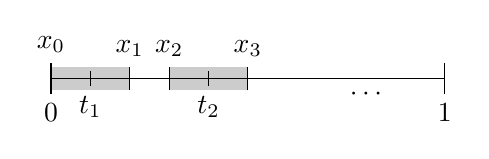
\begin{tikzpicture}
            \fill [black!20] (0,-0.15) rectangle (1,0.15);
            \fill [black!20] (1.5,-0.15) rectangle (2.5,0.15);
            \draw (0,0) -- (5,0);
            \draw (0,-0.2) -- (0,0.2) node [pos=0,below] {$0$} node [pos=1,above] {$x_0$};
            \draw (5,-0.2) -- (5,0.2) node [pos=0,below] {$1$};
            \draw (0.5,-0.1) -- (0.5,0.1) node [pos=0,below] {$t_1$};
            \draw (1,-0.15) -- (1,0.15) node [pos=1,above] {$x_1$};
            \draw (2,-0.1) -- (2,0.1) node [pos=0,below] {$t_2$};
            \draw (1.5,-0.15) -- (1.5,0.15) node [pos=1,above] {$x_2$};
            \draw (2.5,-0.15) -- (2.5,0.15) node [pos=1,above] {$x_3$};
            \node [below] at (4,0) {$ \cdots $};
        \end{tikzpicture}        
    \end{center}
    Outside these intervals, $ f(x)<1/N $. Clearly $ f\le 1 $, so
    \[
        U(f,D)\le 1/N+\frac{\epsilon}{2}<\epsilon.
    \]
\end{example}

\begin{proposition}
    Suppose $f,g:[a,b]\to\mathbb R$ are integrable, then
    \begin{enumerate}
        \item If $\lambda\in\mathbb R$, then $f+\lambda g$ is integrable and
        $$\int_a^bf(x)+\lambda g(x)\,\mathrm dx=\int_a^bf(x)\,\mathrm dx+\lambda\int_a^bg(x)\,\mathrm dx.$$
        \item For any $c\in [a,b]$, $f|_{[a,c]},f|_{[c,b]}$ are integrable and
        $$\int_a^cf(x)\,\mathrm dx+\int_c^bf(x)\,\mathrm dx=\int_a^bf(x)\,\mathrm dx.$$
        \item If $f\ge g$ on $[a,b]$, then
        $$\int_a^bf(x)\,\mathrm dx\ge\int_a^bg(x)\,\mathrm dx.$$
        \item $|f|$ is integrable and
        $$\left|\int_a^bf(x)\,\mathrm dx\right|\le\int_a^b|f(x)|\,\mathrm dx.$$
        \item $fg$ is integrable.
    \end{enumerate}
\end{proposition}
\begin{proof}
    Exercise.
\end{proof}
\begin{notation}
    If $a>b$, let 
    \[
        \int_{a}^{b} f(x) \,\mathrm{d}x = - \int_{b}^{a} f(x) \,\mathrm{d}x
    \]
    and if $a=b$, then let 
    \[
        \int_{a}^{a} f(x) \,\mathrm{d}x=0.
    \]
\end{notation}
With this convention, if $|f|\le K$, then 
\[
    \left| \int_{a}^{b} f(x) \,\mathrm{d}x \right| \le K|b-a|.
\]

\subsection{Fundamental Theorem of Calculus}
Let $f:[a,b]\to \mathbb{R} $ be bounded ($ |f(x)|\le K $) and integrable. Define 
\[
    F(x) = \int_{a}^{x} f(t) \,\mathrm{d}t.
\]
\begin{theorem}\label{thm:5.7}
    $F$ is continuous.
\end{theorem}
\begin{proof}
    Note that 
    \[
        \left| F(x+h)-F(x) \right|  = \left| \int_{x}^{x+h} f(t) \,\mathrm{d}t \right| \le K|h|.
    \]
    let $h\to 0$ gives the result.
\end{proof}

\begin{theorem}[FTC]\label{thm:5.8}
    If $f$ is continuous at $x$, then $F$ is differentiable at $x$ and
    \[
        F'(x)=f(x).
    \] 
\end{theorem}
\begin{proof}
    Need to consider (for $ x+h\in [a,b],h\neq 0 $) that
    \begin{align*}
        \left| \frac{F(x+h)-F(x)}{h}-f(x) \right|&= \frac{1}{|h|}\left| \int_{x}^{x+h} f(t) \,\mathrm{d}t - h f(x) \right| \\ 
        &= \frac{1}{|h|} \left| \int_{x}^{x+h} f(t)-f(x) \,\mathrm{d}t \right| .
    \end{align*}
    Since $f$ is continuous at $x$, given $ \epsilon>0,\ \exists \delta>0  $ such that if $ |t-x|<\delta $, then $ |f(t)-f(x)|<\epsilon$. So if $ |h|<\epsilon $, 
    \[
        \frac{1}{|h|} \left| \int_{x}^{x+h} f(t)-f(x) \,\mathrm{d}t \right|\le \frac{1}{|h|} \epsilon |h| = \epsilon.
    \]
    Which means 
    \[
        \lim_{h \to 0} \frac{F(x+h)-F(x)}{h} = F'(x) = f(x).\qedhere
    \]
\end{proof}
\begin{example}
    Let 
    \[
        f(x) = \begin{cases}
        -1 &x\in [-1,0]\\
        1 &x\in [0,1]\\
        \end{cases} 
    \]
    Check that $f$ is integrable. Check also that $F(x)=-1+|x|$ is differentiable on $ [-1,1]\setminus \{0\} $.
\end{example}
\begin{corollary}[Integration is the inverse of differentiation]
    If $f=g'$ is continuous on $[a,b]$, then 
    \[
        \int_{a}^{x} f(t) \,\mathrm{d}t = g(x)-g(a),\quad \forall x\in [a,b].
    \]
\end{corollary}
\begin{proof}
    By FTC, $(F-g)'=0$ on $ [a,b] $, so it is constant. Since $F(a)=0$, $ F(x)=g(x)-g(a) $ as claimed.
\end{proof}

\begin{note}
    Every continuous function has an \textbf{indefinite integral} or \textbf{anti-derivative} written in 
    \[
        \int f(x) \,\mathrm{d}x
    \]
    which is determined up to a constant.
\end{note}
\begin{remark}
    We actually have solved the ODE 
    \[
        \begin{cases}
         y'(x)=f(x),\\
         y(a)=y_0.\\
        \end{cases}
    \]
\end{remark}

\begin{corollary}[Integration by Part]
    Suppose $f,g:[a,b]\to\mathbb R$ are continuously differentiable on $[a,b]$, then
    $$\int_a^bg^\prime(t)h(t)\,\mathrm dt=g(b)h(b)-g(a)h(a)-\int_a^bg(t)h^\prime(t)\,\mathrm dt.$$
\end{corollary}
\begin{proof}
    By product rule, $ (fg)'=f'g+fg' $ and by FTC,
    \[
        f(b)g(b)-f(a)g(a)=\int_{a}^{b} f'(x)g(x) \,\mathrm{d}x + \int_{a}^{b} f(x)g'(x) \,\mathrm{d}x.\qedhere
    \]
\end{proof}
\begin{corollary}[Integration by substitution]
    Suppose $f:[a,b]\to\mathbb R$ is continuous and $g:[\alpha,\beta]\to\mathbb R$ is continuously differentiable on $ [\alpha,\beta] $, and $g(\alpha)=a, g(\beta)=b$, then
    $$\int_a^bf(x)\,\mathrm dx=\int_\alpha^\beta f(g(t))g^\prime(t)\,\mathrm dt.$$
\end{corollary}
\begin{proof}
    Set 
    \[
        F(x) = \int_{a}^{x} f(t) \,\mathrm{d}t,\quad h(t) = F(g(t)).
    \]
    Then
    \[
        \int_{\alpha}^{\beta} f(g(t))g'(t) \,\mathrm{d}t = \int_{\alpha}^{\beta} F'(g(t))g'(t) \,\mathrm{d}t = \int_{\alpha}^{\beta} h'(t) \,\mathrm{d}t = h(\beta)-h(\alpha),
    \]
    which is exactly $ F(b)-F(a) $.
\end{proof}

We introduce a definition that makes our lives easier:
\begin{definition}
    $ f: \mathbb{R} \ni E \to \mathbb{R}  $ is said to be $ C^k,\ k\in \mathbb{N} $, if $ f^{(i)} $ exists and is continuous for all $i=1,\dots,k$. We say $f$ is $ C^\infty $ if $ f^{(n)} $ exists and is continuous for all $n\in \bbN$.
\end{definition}

\begin{theorem}[Taylor's theorem with integral remainder]
    If $f$ is $C^n$ for $ x\in [0,h] $, then 
    \[
        f(h) = \sum_{k=0}^{n-1}\frac{h^k f^{(k)}(0)}{k!} + R_n,
    \]
    where $ R_n $ is the \textbf{integral remainder}
    \[
        R_n = \frac{h^n}{(n-1)!}\int_{0}^{1} (1-t)^{n-1}f^{(n)}(th) \,\mathrm{d}t.
    \]
\end{theorem}
\begin{proof}
    By substituting $ u=th $, 
    \[
        R_n = \frac{1}{(n-1)!}\int_{0}^{h} (h-u)^{n-1}f^{(n)}(u) \,\mathrm{d}u .
    \]
    Integrating by parts we get 
    \begin{align*}
        R_n&= -\frac{h^{n-1}f^{(n-1)}(0)}{(n-1)!}+\frac{1}{(n-2)!} \int_{0}^{h} (h-u)^{n-2}f^{(n-1)}(u) \,\mathrm{d}u\\ &= -\frac{h^{n-1}f^{(n-1)}(0)}{(n-1)!}+R_{n-1}\\ 
        &= \cdots = - \sum_{k=1}^{n-1}\frac{h^kf^{(k)}(0)}{k!} + \int_{0}^{h} f'(u) \,\mathrm{d}u\\ 
        &= - \sum_{k=1}^{n-1}\frac{h^kf^{(k)}(0)}{k!} +f(h)-f(0).\qedhere
    \end{align*}
\end{proof}
We can use this to get Cauchy and Lagrange forms of remainders. However, note that the proof above uses continuity of $f^{(n)}$, not just mere existence as in section 3. But first,
\begin{theorem}[Integral Mean Value Theorem]
    If $ f,g:[a,b]\to \mathbb{R}  $ are continuous with $ g(x)\neq 0 $, then $ \exists c\in (a,b) $ such that 
    \[
        \int_{a}^{b} f(x)g(x) \,\mathrm{d}x = f(c) \int_{a}^{b} g(x) \,\mathrm{d}x.
    \]
\end{theorem}
\begin{note}
    If take $ g(x)=1 $ then 
    \[
        \int_{a}^{b} f(x) \,\mathrm{d}x = f(c)(b-a),
    \]
    which is the integral form of differential MVT.
\end{note}
\begin{proof}
    Use Cauchy's MVT on 
    \[
        F(x) = \int_{a}^{x} f(x)g(x) \,\mathrm{d}t,\quad G(x)=\int_{a}^{x} g(t) \,\mathrm{d}t,
    \]
    $ \exists c\in (a,b) $ such that 
    \begin{align*}
        &(F(b)-F(a))G'(c)=F'(c)(G(b)-G(a))\\ 
        \Longrightarrow & \left( \int_{a}^{b} f(x)g(x) \,\mathrm{d}x \right)g(c)=f(c)g(c)\left( \int_{a}^{b} g(x) \,\mathrm{d}x \right).
    \end{align*}
    Since $g(c)\neq 0$ by assumption, the result follows.
\end{proof}

Start from 
\[
    R_n = \frac{h^n}{(n-1)!}\int_{0}^{1} (1-t)^{n-1}f^{(n)}(th) \,\mathrm{d}t,
\]
by applying MVT with $g=1$ we get
\[
    R_n = \frac{h^n (1-\theta)^{n-1}}{(n-1)!}f^{(n)}(\theta h),\quad \theta\in (0,1),
\]
the Cauchy form. To get Lagrange, apply MVT with $ g(t)=(1-t)^{n-1}>0 $ for $ t\in (0,1)$
\[
    R_n=\frac{h^n}{(n-1)!} f^{(n)}(\theta h) \int_{0}^{1} (1-t)^{n-1} \,\mathrm{d}t = \frac{h^n }{n!}f^{(n)}(\theta h),\quad \theta\in (0,1). 
\]

\begin{theorem}[Newton's Binomial Theorem]\label{gen_bin}
    For $x\in (-1,1)$, $P(x)$ converges to $(1+x)^s$.
\end{theorem}
\begin{lemma}
    $$k\binom{s}{k}=s\binom{s-1}{k-1},\binom{s}{k-1}+\binom{s}{k}=\binom{s+1}{k}$$ 
\end{lemma}
\begin{proof}
    Trivial.
\end{proof}
\begin{proof}[Proof of Theorem \ref{gen_bin}]
    By termwise differentiation,
    $$(1+x)P^\prime(x)=(1+x)\sum_{i=0}^\infty i\binom{s}{i}x^{i-1}=sP(x)$$
    by the preceding lemma.
    So consider $h(x)=(1+x)^{-s}P(x)$, so $h^\prime(x)=0$ by the differential equation we obtained above, hence $h$ is constant in $(-1,1)$, hence $h\equiv h(0)=1$.
    Therefore $P(x)=(1+x)^s$ for each $x\in (-1,1)$.
\end{proof}

\subsection{Improper integrals}

Our definition of integral
$$\int_a^bf(x)\,\mathrm dx$$
requires $a,b<\infty$ and $f$ is defined and bounded in $[a,b]$.
But we'd also like to think about things like
$$\int_1^\infty\frac{\mathrm dx}{x^2+1},\int_0^1\frac{\mathrm dx}{\sqrt{x}}$$
which are not defined in our previous definition of integral.

Suppose $f:[a,b)\to\mathbb R$ is continuous and $b\in\mathbb R\cup\{\infty\}$.
Then if $x\in [a,b)$, then
$$\int_a^xf(t)\,\mathrm dt$$
is well-defined since $f$ is continuous on $[a,x]$.

\begin{definition}
    If $f:[a,b)\to\mathbb R$ is continuous and
    $$\lim_{x\to b^-}\int_a^x f(t)\,\mathrm dt$$
    exists and equals to some $\ell\in\mathbb R$, we define
    $$\int_a^bf(t)\,\mathrm dt=\ell $$
    and say that this integral \textit{exists} and \textit{converges}.
    If this limit does not exist, we say the integral diverges.

    Similarly, if $f:(a,b]\to\mathbb R$ is continuous and
    $$\lim_{x\to a^+}\int_x^bf(t)\,\mathrm dt$$
    exists and equals to $\ell $, then we define
    $$\int_a^bf(t)\,\mathrm dt=\ell $$
    and say that this integral converges.
    Otherwise we say this integral diverges.
\end{definition}
Note that by FTC this definition (whenever the integral converges) does coincide with our original definition of integrals.
\begin{remark}
    The last part is NOT the same as saying that the symmetric limit
    \[
        \lim_{R \to \infty} \int_{-R}^{R} f(x) \,\mathrm{d}x
    \]
    exists. It is a stronger statement. e.g. 
    \[
        \int_{-R}^{R} x \,\mathrm{d}x=0
    \]
    but $ \int_{0}^{\infty} x \,\mathrm{d}x $ and $ \int_{-\infty}^{0} x \,\mathrm{d}x $ both diverge. In order to make this a thing, we need to introduce concept of \textbf{principal value} and that is beyond this course.
\end{remark}

\begin{example}
    Consider the integral
    $$\int_1^\infty t^{-s}\,\mathrm dt$$
    Then for $s>1$, then integral converges and equals $1/(s-1)$, and it diverges for $s\le 1$.
    Similarly
    $$\int_0^1 t^{-s}\,\mathrm dt$$
    converges iff $s<1$.
\end{example}
Even more generally,
\begin{definition}
    If $f:(a,b)\to\mathbb R$ is continuous, then choose $c\in (a,b)$, then if
    $$\int_a^cf(t)\,\mathrm dt,\int_c^bf(t)\,\mathrm dt$$
    both converge, then we say the integral of $f(t)$ over $(a,b)$ converges and
    $$\int_a^bf(t)\,\mathrm dt=\int_a^cf(t)\,\mathrm dt+\int_c^bf(t)\,\mathrm dt$$
\end{definition}
Note that this definition (both the convergence and the value of the integral) does not depend on the choice of $c$.

\begin{remark}
    The second definition is NOT the same as saying that, for example in $(-\infty,\infty) $ case, thatx the symmetric limit
    \[
        \lim_{R \to \infty} \int_{-R}^{R} f(x) \,\mathrm{d}x
    \]
    exists. It is a stronger statement.
\end{remark}
\begin{example}
    We have
    $$\int_{-\infty}^\infty\frac{\mathrm dx}{1+x^2}=\int_{-\infty}^0\frac{\mathrm dx}{1+x^2}+\int_{0}^\infty\frac{\mathrm dx}{1+x^2}=\pi$$
    But
    $$\int_{-\infty}^\infty t\,\mathrm dt$$
    does not converge since
    $$\int_0^\infty f(t)\,\mathrm dt$$
    does not converge.
    $$\int_0^\infty t^{-s}\,\mathrm dt=\int_0^1 t^{-s}\,\mathrm dt+\int_1^\infty t^{-s}\,\mathrm ds$$
    never converges for any value of $s$.
\end{example}
\begin{sprop}
    If $f,g\ge 0$ for $x\in [a,b)$ and $ f(x)\le Kg(x),\ \forall x\ge a, K $ constant, then 
    \[
        \int_{a}^{b} g(x) \,\mathrm{d}x \text{ converges} \Longrightarrow \int_{a}^{b} f(x) \,\mathrm{d}x \text{ converges},
    \]
    and 
    \[
        \int_{a}^{b} f(x) \,\mathrm{d}x\le K \int_{a}^{b} g(x) \,\mathrm{d}x.
    \]
\end{sprop}
\begin{example}
    Since $ e^{-x^2/2}\le e^{x/2} $ for $x\ge 1$, the integral over $ [0,\infty) $ of the first function is convergent.
\end{example}
\begin{remark}
    We know that if $ \sum a_n $ converges then $ a_n\to 0 $. We have to be a little more careful with improper integrals. Construct a counterexample yourself!
\end{remark}

\begin{theorem}[The Integral Test]
    Suppose $f:[1,\infty)\to[0,\infty)$ is continuous and decreasing, then
    $$\sum_{n=1}^\infty f(n) \text{ converges} \Longleftrightarrow \int_1^\infty f(t)\,\mathrm dt \text{ converges}$$
    and 
    \[
        \sum_{n=1}^\infty f(n) \text{ diverges} \Longleftrightarrow \int_1^\infty f(t)\,\mathrm dt \text{ diverges}.
    \]
    Also as $ n\to \infty $, 
    \[
        \sum_{r=1}^{n}f(r)-\int_{1}^{n} f(x) \,\mathrm{d}x\to \ell 
    \]
    such that $ 0\le \ell \le f(1) $.
\end{theorem}
\begin{proof}
    Clearly that if $ n-1\le x\le n $, then $ f(n-1)\ge f(x)\ge f(n) $. Integrating gives 
    \[
        f(n-1)\ge \int_{n-1}^{n} f(x) \,\mathrm{d}x\ge f(n).
    \]
    Adding from $2$ to $n$ we get 
    \[
        \sum_{r=1}^{n-1}f(r) \ge \int_{1}^{n} f(x) \,\mathrm{d}x\ge \sum_{r=2}^{n}f(r).
    \]
    The first claim follows. For the proof of the second one, let
    \[
        \phi(n) = \sum_{r=1}^{n}f(r)-\int_{1}^{n} f(x) \,\mathrm{d}x.
    \]
    Observe that 
    \[
        \phi(n)-\phi(n-1) = f(n)-\int_{n-1}^{n} f(x) \,\mathrm{d}x\le 0
    \]
    by the first inequality. Also 
    \[
        0\le \phi(n)\le f(1)
    \]
    by the second inequality. The result follows.
\end{proof}